\documentclass[a4paper,12pt]{article}

\usepackage[left=25mm, right=25mm, top=25mm, bottom=25mm]{geometry}

\usepackage{amsmath}
\usepackage{amssymb}
\usepackage{amsfonts}
\usepackage[style=iso]{datetime2}
\usepackage[explicit]{titlesec}
\usepackage{amsthm}
\usepackage{mathrsfs}
\usepackage{array}
\usepackage{graphicx}
\usepackage{mathtools} % Provides \mathrlap command
\usepackage{xparse}
\usepackage{float}
\usepackage[skip=1em,indent]{parskip}
\usepackage{caption}
\usepackage[colorlinks=true, linkcolor=black]{hyperref}
\usepackage{tocloft}
\usepackage{enumitem}
\usepackage[toc, page]{appendix}
\usepackage{accents}
\usepackage[perpage, symbol*]{footmisc} % for dagger footnotes
\DefineFNsymbols{sym}{\textdagger \textdaggerdbl \textsection \textparagraph %
{\textdagger\textdagger} {\textdaggerdbl\textdaggerdbl} %
{\textsection\textsection} {\textparagraph\textparagraph}}
\setfnsymbol{sym}

\usepackage{tikz}
\tikzset{>=latex} % for LaTeX arrow head
\usepackage{pgfplots} % for the axis environment
\usetikzlibrary{calc,decorations.markings}

\pgfplotsset{compat=1.18, every tick label/.append style={font=\footnotesize}}

\graphicspath{ {./Images/} }

\makeatletter
\def\th@plain{%
  \thm@notefont{}% same as heading font
  \itshape % body font
}
\def\th@definition{%
  \thm@notefont{}% same as heading font
  \normalfont % body font
}
\makeatother

\newcommand*\diff{\mathop{}\!d} % for the differential in integrals
% ---------------- %
\ExplSyntaxOn %* This command is for row vectors; unstarred version has no delimiter scaling for inline; starred version has delimiter scaling for display
\seq_new:N \l_user_rvec_seq

% expl3 worker (does the splitting/formatting)
\cs_new_protected:Npn \dbacc_rvec:n #1
 {
  \seq_clear:N \l_user_rvec_seq
  \seq_set_split:Nnn \l_user_rvec_seq { , } { #1 }
  \seq_use:Nn \l_user_rvec_seq { \enspace }
 }

% plain-name wrapper (no ':' in its name) — safe to call outside ExplSyntaxOn
\cs_new_protected:Npn \dbaccrvec #1 { \dbacc_rvec:n { #1 } }

% user-level \rvec interface (star + optional size + mandatory arg)
\NewDocumentCommand \rvec { s o m }
 {
  \IfBooleanTF{#1}
    { \left[\,\dbaccrvec{#3}\,\right] } % starred -> automatic \left...\right
    { \IfValueTF{#2}
        { \mathopen{#2[}\,\dbaccrvec{#3}\,\mathclose{#2]} } % sized optional arg
        { [\,\dbaccrvec{#3}\,] } % default small delimiters
    }
 }
\ExplSyntaxOff
% ---------------- %
\newcommand{\R}{\mathbb{R}}
\newcommand{\C}{\mathbb{C}}
\newcommand{\Z}{\mathbb{Z}}

\NewCommandCopy{\oldIm}{\Im}
\renewcommand{\Im}{\mathop{\oldIm\mathfrak{m}}}
\NewCommandCopy{\oldRe}{\Re}
\renewcommand{\Re}{\mathop{\oldRe\mathfrak{e}}}

\newcommand{\overbar}[1]{\mkern 1.5mu\overline{\mkern-1.5mu#1\mkern-1.5mu}\mkern 1.5mu}

\DeclareMathOperator{\Res}{Res}
% ---------------- %
\newcommand{\ihat}{\boldsymbol{\hat{\imath}}}
\newcommand{\jhat}{\boldsymbol{\hat{\jmath}}}
\newcommand{\khat}{\boldsymbol{\hat{k}}}
% ---------------- %

\newtheorem{theorem}{Theorem}
\newtheorem{lemma}[theorem]{Lemma}
\newtheorem{proposition}[theorem]{Proposition}
\newtheorem{corollary}{Corollary}[theorem]

\theoremstyle{definition}
\newtheorem{definition}[theorem]{Definition}
\newtheorem{example}[theorem]{Example}

% \setlength{\cftsecnumwidth}{3em}

\begin{titlepage}
\title{Introduction to Differential Forms}
\author{Abdul Musthakin}
\date{October 2025}
\end{titlepage}

% \renewcommand{\thesection}{\Roman{section}}

\allowdisplaybreaks

\setlength{\parindent}{0pt}

\begin{document}
\maketitle

\tableofcontents

\pagebreak

\section{Introduction \& Motivation}

Understanding what an integral means, in a general sense, is not particularly difficult.
Given a function, it is pretty easy to draw it as a curve on a graph.
By looking at its graph, and choosing some interval on the $x$-axis, we can see the area between the curve and the $x$-axis.
This (signed) area is what is calculated by an integral.
\begin{figure}[H]
\centering
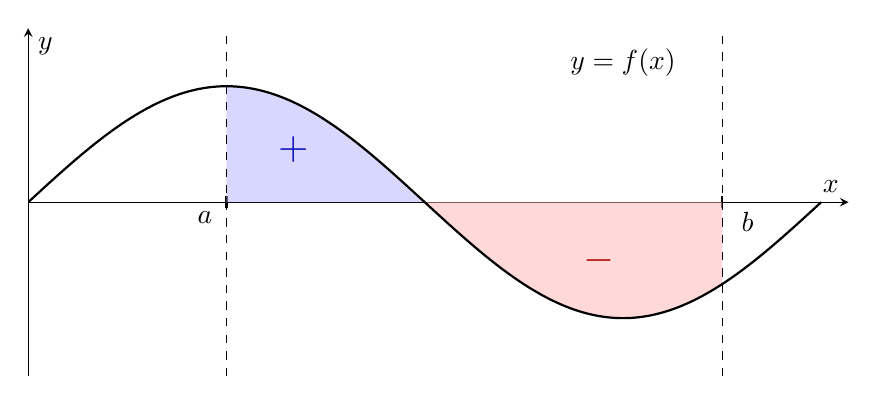
\begin{tikzpicture}
\begin{axis}[
    width=12cm,
    height=6cm,
    axis lines=middle,
    xlabel={$x$},
    ylabel={$y$},
    xmin=0, xmax=6.5,
    ymin=-1.5, ymax=1.5,
    xtick={1.5708, 5.49779},
    xticklabels={},
    ytick=\empty,
    samples=200,
    domain=0:2*pi,
    enlargelimits=false,
    tick style={black, thick},
    major tick length=0.15cm,
]

% Labels for a and b
\node[below] at (axis cs:1.4, 0) {$a$};
\node[below] at (axis cs:5.7, 0) {$b$};

% Shaded area for positive region (a to π)
\addplot[fill=blue!30, opacity=0.5, domain=1.5708:3.14159, draw=none] 
    {sin(deg(x))} \closedcycle;

% Shaded area for negative region (π to b)
\addplot[fill=red!30, opacity=0.5, domain=3.14159:5.49779, draw=none] 
    {sin(deg(x))} \closedcycle;

% The sin(x) function
\addplot[black, thick, domain=0:2*pi] {sin(deg(x))};

% Vertical lines at x=a and x=b
\addplot[dashed, black] coordinates {(1.5708, -1.5) (1.5708, 1.5)};
\addplot[dashed, black] coordinates {(5.49779, -1.5) (5.49779, 1.5)};

% Label for the function
\node[above, black] at (axis cs:4.71239, 1) {$y = f(x)$};

% Labels for areas
\node[blue!70!black, font=\Large] at (axis cs:2.1, 0.45) {$+$};
\node[red!70!black, font=\Large] at (axis cs:4.52, -0.5) {$-$};

\end{axis}
\end{tikzpicture}
\caption{A definite integral}
\label{fig:definite_integral_sin}
\end{figure}
The area illustrated by the above figure is given by
\begin{equation*}
    \int_{a}^{b} f(x) \diff x.
\end{equation*}
Now, everything that was just stated has many asterisks.
We can have functions that cannot be integrated, or at least, not in the `usual' sense.
Even if we can integrate a function, we might not be able to get our integral (and thus desired area) in terms of functions that we are used to.
Even if we ignore all of that, there is plenty of theory regarding how we define integrals -- extending and generalizing to different applications.
So it turns out that integrals are not that simple, but their idea is.

The above refers specifically to definite integrals, and so too will further discussion.
It would thus be useful to have a brief mention of indefinite integrals for the sake of completeness.
An indefinite integral of some function $f$ is itself not a number, nor even a function.
It is a class of functions,\footnote{An equivalence class.} whose shared property is that their derivative is $f$.
A member of this class is referred to as an antiderivative of $f$, and it can be written as
\begin{equation*}
    F(x) \coloneq c + \int_{a}^{x} f(t) \diff t,
\end{equation*}
where $a$ and $c$ are some constants.
Since any antiderivative (and thus the indefinite integral) of a function can be rewritten in terms of a definite integral, there is nothing regarding the former concept that warrants its mention in the discussions ahead.

Consider the notation we use for integrals.
We have a unique symbol, $\int$, to always know when we are integrating.
We have the integrand after that, which is what we are integrating.
Also, we have the start and end points of our interval which we are integrating over.
Finally, we have something on the end.
It is definitely not useless, as it tells us what variable we are integrating with respect to.
For instance, it is true that
\begin{equation*}
    \int_{a}^{b} f(x) \diff x = \int_{a}^{b} f(t) \diff t = \int_{a}^{b} f(u) \diff u,
\end{equation*}
just as it is true that
\begin{equation*}
    \sum_{i=1}^{n} f(i) = \sum_{j=1}^{n} f(j) = \sum_{k=1}^{n} f(k).
\end{equation*}
The exact symbol we use for the variable does not matter; they are just labels for the same thing.
Now, in the context of sums, you can simply expand out to show that they are the same thing.
They all refer to $f(1) + f(2) + f(3) + \ldots + f(n)$.
It is not so straightforward for integrals, but the idea holds.
We could leave it at that, and say that the differential is just a part of the notation that conveys some useful information.
There is much more to it than that, however.

The word `differential' has many meanings in mathematics, and it can refer to completely different concepts in different fields (or even in the same field).
One thing that it can refer to is an infinitesimal -- a number closer to zero than any real number that is not itself zero.
Leibniz was the first to coin the term for that usage, although the idea of infinitesimals date back to \href{https://plato.stanford.edu/entries/continuity/}{ancient Greek mathematicians}.

Early developments in calculus throughout the 17th and 18th centuries by the likes of Newton and Leibniz were noticeably reliant on the idea of infinitesimals.
That itself was not a bad thing, but that the lack of rigour was.
We would see the development of a more rigourous foundation of calculus by mathematicians in the 19th century, particularly Cauchy.
Infinitesimals would be left in favour of limits, and the latter is the formulation that is universally taught in schools.
\begin{figure}[H]
\centering
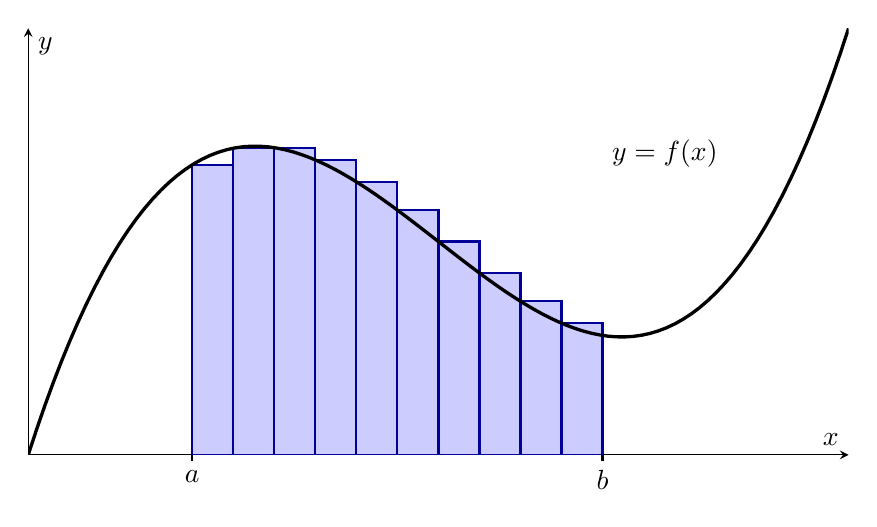
\begin{tikzpicture}
\begin{axis}[
    width=12cm,
    height=7cm,
    axis lines=middle,
    xlabel={$x$},
    ylabel={$y$},
    xmin=0, xmax=10,
    ymin=0, ymax=100,
    xtick={2, 7},
    xticklabels={$a$, $b$},
    ytick=\empty,
    samples=100,
    domain=0:10,
    enlargelimits=false,
    tick style={black, thick},
    major tick length=0.15cm,
    xticklabel style={font=\normalsize},
]


% Draw Riemann sum rectangles (left endpoint)
\foreach \i in {0,...,9} {
    \pgfmathsetmacro{\xleft}{2 + \i*0.5}
    \pgfmathsetmacro{\xright}{\xleft + 0.5}
    \pgfmathsetmacro{\height}{-15*(\xleft-5) + (\xleft-5)^3 + 50}
    \addplot[fill=blue!20, draw=blue!60!black, thick] coordinates {
        (\xleft, 0) (\xleft, \height) (\xright, \height) (\xright, 0)
    } -- cycle;
}

% The curve
\addplot[black, very thick, domain=0:10] {-15*(x-5) + (x-5)^3 + 50};

% Label for the function
\node[above right, black] at (axis cs:7, 65) {$y = f(x)$};

\end{axis}
\end{tikzpicture}
\caption{Riemann sum approximation of an integral}
\label{fig:riemann_sum}
\end{figure}
This information about differentials allows us to view the one attached to every integral in way beyond just useful notation.
Putting the formalism and rigourous defintions of integrals aside, they are fancy sums.
The area under a graph can be approximated by rectangles, as is shown by the above figure.
As the width of the rectangles decrease, the sums \href{https://commons.wikimedia.org/wiki/File:Riemann_sum_(leftbox).gif}{get closer} to the actual area under the curve.
That is, the limit of this sum is an integral.

Instead of thinking about it in terms of limits, we can imagine summing an infinite number of rectangles with infinitesimal width.
The height of a rectangle at some value of $x$ can be given by $f(x)$, so if the integral sums over areas, the $dx$ is the infinitesimal width.
This is all very impercise and non-technical language.
However, it is enough to give us an intuitive feel of what an integral is and what the differential that is always attached to it means.

There is more to the peculiar symbol, though, and integrals are probably not the first place one would have spotted them.
That would instead be with regard to derivatives.
Indeed, the notation $dy/dx$ -- also attributed to Leibniz -- is very commonly used to denote the derivative of $y$ with respect to $x$.
When it is first taught to students at school, the warning will be given that it does not represent a fraction.
It just looks like a fraction, and treating it like a fraction works out almost all the time.

The resemblence it has to a ratio between two quantities is no coincidence, as Leibniz intended it to be just that: a ratio of infinitesimals.
The symbols $dx$ and $dy$ were used to represent infinitely small changes in $x$ and $y$ respectively.
Whilst we have, for the most part, left these impercise notions behind, they will prove to be somewhat useful in understanding these symbols.\footnote{At the end of the day, the symbols mean whatever we want as long as it consistent with the rest of our maths. That is why I gave the easy way out at the beginning, saying that the differential symbol in the integral can just be considered a part of the notation. However, as is being demonstrated, we can go further.}

\section{Differential of a Function}

Firstly, consider the fact that the derivative has many different notations.
The derivative of a function $f$ at $x$ may be expressed as $f'(x)$.
It follows that
\begin{equation*}
    \frac{dy}{dx} = f'(x).
\end{equation*}
This is just equating two things that are defined to mean the exact same thing.
Now, although the left-hand side is not a fraction, what if we rewrote the equation as follows?
\begin{equation*}
    dy = f'(x) \diff x
\end{equation*}
The right-hand side now looks exactly like an integrand.
This looks promising, but we did say beforehand that $dy/dx$ is not a fraction.
So, are we allowed to do that?
No. The symbols $dx$ and $dy$ have not been given a meaning outside of when they appear in $dy/dx$, so it makes no sense to seperate them.
However, when something does not have meaning, we can always attempt to give it one and see where that leads us.

First, let $\Delta x$ be some real number, just as $x$ is.
Then, we can call $df$ the differential of $f$, a function of $x$.
The differential itself is a function of both $x$ and $\Delta x$, is defined as
\begin{equation*}
    df(x, \Delta x) \coloneq f'(x) \Delta x.
\end{equation*}
What was the point of that?
We went from performing an algebraic manipulation in a situation where it does not make sense, to creating a perfectly fine definition.
Since we have made it clear that $df$ is a function of two variables, we can write $df(x, \Delta x)$ as $df(x)$ or even $df$ (we are not changing the meaning).
The differential of the function $f(x) = x$ is given by
\begin{equation*}
    dx = 1 \cdot \Delta x = \Delta x.
\end{equation*}
Even though $dx$ is technically a function of $x$ still, the value of $x$ will not affect it at all, so we may just write $dx = \Delta x$.
With this, and by letting $y = f(x)$, we can rewrite our equation as
\begin{equation*}
    dy = f'(x) \diff x.
\end{equation*}
This looks exactly like what we already had, but now we have reached it by valid means.
We see that the differential $dy$ is defined in terms of $x$ and $dx$, and the differential $dx$ is essentially just some real number.
If we desired, we could go further to obtain $dy/dx = f'(x)$, but this can lead to confusion.
By that equation, $f'(x)$ equals a ratio of differentials that have each been seperately defined.
However, $f'(x)$ is can be expressed with Leibniz's notation as $dy/dx$ -- which is not a ratio.\footnote{We cannot redefine the derivative to be a ratio of our two differentials. Their definitions involve the derivative, so it would be circular. Instead, view it as evidence for the self-consistency of Leibniz's notation}
This is just something to note.

We have now obtained our third interpretation of the differential, a function of two real numbers $x$ and $\Delta x$.
This can be extended to higher-order differentials, as well as to the differentials of multivariable functions.
Its usefulness is in the fact that it represents the principal part of the change of a function.
To see what that exactly means, consider some function\footnote{Technically, $f$ is the function and $f(x)$ is the value of the function at $x$.} $y=f(x)$ between two points $x$ and $x + \Delta x$.
Let $x$ be fixed.
The change in $x$ values is $\Delta x$ and the change in $y$ values is $\Delta y \coloneq f(x + \Delta x) - f(x)$.

By the definition of the derivative, $\Delta y / \Delta x \to f'(x)$ as $\Delta x \to 0$.
This means that for small $\Delta x$, we have $\Delta y / \Delta x \approx f'(x)$.
If the difference (or error) is $\varepsilon$, then $\Delta y / \Delta x = f'(x) + \varepsilon$.
Rearranging gives us
\begin{align*}
    \Delta y &= (f'(x) + \varepsilon) \Delta x \\
    &= f'(x) \Delta x + \varepsilon \Delta x \\
    &= dy + \varepsilon \Delta x.
\end{align*}
The change in $y$ is equal to a linear function of $\Delta x$, $dy$, plus a (generally) nonlinear error term.
Thus, $dy$ is the linear (or principal) part of $\Delta y$.
As $\Delta x \to 0$, the error term goes to zero, so $dy \to \Delta y$, and $\Delta y \approx dy$ for small $\Delta x$.

Let us look at one use case of this: approximating the values of functions.
What is the value of $\sqrt{90}$?
Since the function $y = \sqrt{x}$ is strictly increasing, we know that $\sqrt{90}$ will be between $\sqrt{81}=9$ and $\sqrt{100}=10$.
Let $x = 100$ and $\Delta x = -10$, so that $x + \Delta x = 90$.
Thus, $\Delta y = \sqrt{90} - \sqrt{100} = \sqrt{90} - 10$.
This means that $10 - \Delta y$ is the exact value of $\sqrt{90}$, but we do not know what $\Delta y$ is.
Our approximation from before comes in handy here.

The derivative of $\sqrt{x}$ is given by
\begin{equation*}
    f'(x) = \frac{1}{2\sqrt{x}}.
\end{equation*}
At $x=100$, we have $f'(x) = 1/20 = 0.05$.
This is all we need for our approximation.
\begin{align*}
    \sqrt{90} &= \Delta y + 10 \\
    &\approx dy + 10 \\
    &= f'(10) \Delta x + 10 \\
    &= 0.05 \cdot -10 + 10 \\
    &= 9.5
\end{align*}
The actual value of $\sqrt{90}$ is $9.47213595\ldots$, so we were just 0.62\% off.
The computations were incredibly easy, which is the case as long as we have nice values of the function and its derivative to work with.
We can illustrate the efficacy of this method with a diagram. 
\begin{figure}[H]
\centering
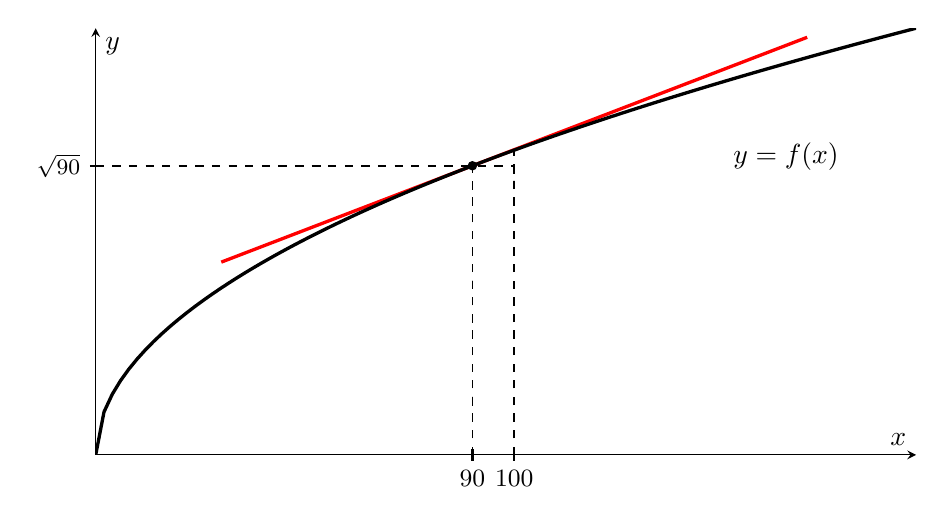
\begin{tikzpicture}
\begin{axis}[
    width=12cm,
    height=7cm,
    axis lines=middle,
    xlabel={$x$},
    ylabel={$y$},
    xmin=0, xmax=196,
    ymin=0, ymax=14,
    xtick={90, 100},
    xticklabels={90, 100},
    ytick={sqrt(90)},
    yticklabels={$\sqrt{90}$},
    samples=100,
    domain=0:196,
    enlargelimits=false,
    tick style={black, thick},
    major tick length=0.15cm,
    xticklabel style={font=\small},
]

\addplot[red, very thick, domain=30:170] {x/(2*sqrt(90)) + (sqrt(90) - 90/(2*sqrt(90)))};

% The curve
\addplot[black, very thick, domain=0:196] {sqrt(x)};

\draw[fill] (axis cs:{90,sqrt(90)}) circle [radius=1.5pt];
\addplot[black, semithick, dashed, domain=0:100] {sqrt(90)};
\addplot[black, semithick, dashed, domain=0:90] (90, {sqrt(x)});

\addplot[black, semithick, dashed, domain=0:100] (100, {sqrt(x)});

% Label for the function
\node[above right, black] at (axis cs:150, 9) {$y = f(x)$};

\end{axis}
\end{tikzpicture}
\caption{Linear approximation of $\sqrt{90}$}
\label{fig:linaer_approximation}
\end{figure}
We calculated $dy$, the increase in the tangent, as an approximation to $\Delta y$, the increase in the function.
As can be seen from the figure, these are very similar values.
Since $f'(x) \to 0$ as $x \to \infty$ (the curve flattens), this method of approximation gets better for larger square roots.
That does not mean that this method is not useful for other functions, as it is generally applicable to functions that are sufficiently `nice' -- where a discussion on `niceness' is besides the point.

Another example is approximating $\ln 3$.
We know that $\ln e$ is 1, and $e \approx 3$.
Let $x = e$ and $\Delta x = 3 - e$, so that $x + \Delta x = 3$.
Then, $\Delta y = \ln 3 - \ln e = \ln 3 - 1$.
The derivative of $\ln x$ is simply $1/x$, so we have
\begin{equation*}
    \ln 3 \approx \frac{1}{e} \cdot (3 - e) + 1 = \frac{3}{e}.
\end{equation*}
The number $e$ is well-known enough for us to use its value for the approximation, giving us $\ln 3 \approx 1.104$.
The actual value is $1.09861229\ldots$, which means that there is a 0.46\% error.
These approximations are known as linear approximations, and they have a fair bit of applications.
The idea of calculating the linear part of $\Delta y$ can be made more precise with \emph{Taylor's theorem}, though it is not necessary to understand the method itself.

\section{Reinterpreting Formulae}

Now that we have a formal definition of a differential, it would be useful to use what we have to look at commonly-known formulae in this new context.
First is the chain rule for derivatives.
Given two functions $f$ and $g$, the derivative of their composition $f \circ g$ is given by
\begin{equation*}
    f'(g(x)) g'(x).
\end{equation*}
If we write $y = f(g(x))$ and $u = g(x)$, then the previous fact can be rewritten as
\begin{equation*}
    \frac{dy}{dx} = \frac{dy}{du} \frac{du}{dx}
\end{equation*}
using Leibniz's notation.
The latter way is writing is more elegant both in this case, and for compositions of more than two functions.
It reinforces the idea of the derivative being a fraction, even though it is not.
If we were to, however, consider the terms on the RHS as being differentials, then we do have fractions -- which can cancel.
\begin{align*}
    \frac{dy}{du} \frac{du}{dx} = \frac{y'(x) \diff x}{u'(x) \diff x} \frac{u'(x) \diff x}{dx} = y'(x)
\end{align*}
Of course this is not a proof of the chain rule.
It does not show that the fraction $dy/du$ is the same as the derivative of $y$ with respect to $u$, and it does not work when $u'(x) = 0$ wherever we are differentiating at.
Regardless, it shows the chain rule to be intuitively very simple -- just `cancelling' fractions.

Our definition of differentials can also be shown to be insightful with regard to integration by substitution and the method of solving differential equations by seperation of variables.
That would make sense, as they are both linked to the chain rule (with the former being an inverse to some degree).
Given two functions $f$ and $g$, the integration by substitution formula states that
\begin{equation*}
    \int_{a}^{b} f(g(x))g'(x) \diff x = \int_{g(a)}^{g(b)} f(u) \diff u.
\end{equation*}
By making the substitution $u = g(x)$, we know that the differential of $u$ is given by $du = g'(x) \diff x$.
This suggests that the formula above is a literal substitution of one variable with another.
The limits being transferred from $x=a$ and $x=b$ to $u=g(a)$ and $u=g(b)$ make sense as well.\footnote{We could have had the limits on the RHS integral be $x=a$ and $x=b$ if we really wanted. This shows that nothing `actually' changes between the two integrals.}
Without the integral symbols, the equation would just be something that follows directly from the defintion of a differential.
If it were possible to integrate a differential in the sense of it being the whole integrand -- not just integrating a function -- then the formula would be completely trivial.

Now, on to the topic of differential equations.
Let $f$, $g$, and $h$ be functions that satisfy the differential equation
\begin{equation*}
    \frac{dy}{dx} = g(x)h(y),
\end{equation*}
with $y=f(x)$.
If we treat the $dy$ in $dy/dx$ as a differential (which is a bit awkward notationally but valid), then we have a fraction that can be seperated.
Multiplying both sides by $dx$ and dividing by $h(y))$ gives
\begin{equation*}
    \frac{dy}{h(y)} = g(x) \diff x.
\end{equation*}
This is really the same as
\begin{equation*}
    \frac{f'(x)}{h(f(x))} \diff x = g(x) \diff x.
\end{equation*}
Since $dx$ is some real number, we can cancel it out and then integrate both sides with respect to $x$ in order to solve the equation.
However, our integrals will have $dx$ at the end anyway.
What was the point of cancelling them out beforehand?
The $dx$ in an integral is still different from the $dx$ we have defined to be equal to some real number $\Delta x$.
Once again, if we could just integrate the differentials directly, things would be much simpler.

\section{Generalizing Differentials}

As was suggested at the end of the previous section, there is a different way to handle differentials that works well with integration.
Before it is covered, we will consider some other generalisations.
Higher-order derivatives correspond to higher-order differentials.
No new definitions are required.
\begin{equation*}
    d^2 y \coloneq d(dy) = d(f'(x)\diff x) = (df'(x)) \diff x = f''(x) (dx)^2
\end{equation*}
Dividing through by $(dx)^2$ gives an equation very similar to Leibniz's notation for higher-order derivatives.
However, note that it is not a definition (as it would be if we were considering it as just notation).
\begin{equation*}
    \frac{d^2 y}{(dx)^2} = f''(x)
\end{equation*}
If the differential $dx$ itself is a function of $x$, then the expression becomes a bit more complicated.
We must use the product rule.
\begin{equation*}
    d^2 y = f''(x) (dx)^2 + f'(x) \diff^2 x
\end{equation*}
Both cases generalise to third derivatives, fourth derivatives, and so on.
There is not much else interesting to say about them, unlike differentials of multivariable functions.
For some function $y = f(x_1, \ldots, x_n)$ of $n$ independent variables, the partial differential of $y$ with respect to some variable $x_i$ is defined to be
\begin{equation*}
    \frac{\partial y}{\partial x_i} \diff x_i.
\end{equation*}
This is the principal part of the change in $y$ from a change $dx_i$ in $x_i$.
Adding these partial differentials for all the independent variables gives the total differential\footnote{Technically, this and the previous definition are first given in terms of $\Delta x_i$, and it is noted that $dx_i(\Delta x_1, \ldots, \Delta x_n) = \Delta x_i$.} of $y$.
\begin{equation*}
    dy \coloneq \sum_{i=1}^{n} \frac{\partial y}{\partial x_i} \diff x_i
\end{equation*}
This is the principal part of the change in $y$ from the changes in all the variables.
This is approximately equal to the actual change in $y$.
Just as in the case of one variable, we have $\Delta y \approx \diff y$.
We will not be referencing higher-order differentials, but their existence is worth noting as they have their uses elsewhere.

After covering functions of multiple variables, a sensible next step would be to cover functions of vectors.
See Appendix~\ref{appendix:vectors} for necessary background knowledge.

\section{Differential Forms}

WIP

\begin{appendices}

\section{Vectors} \label{appendix:vectors}

An introduction to the concept of vectors usually involve giving examples of vectors -- such as arrows in a plane -- without giving a proper definition of what a vector is in general.
That makes sense, since such a definition is fairly technical and unecessary for simply working with vectors.
The technical definition is that a vector is an element of a vector space, but that alone simply replaces one question with another.
It follows that a definition of a vector space is now required.

We know that ordered pairs of real numbers are examples of vectors, so we can work from there.
The notation $\R^2$ is a shorthand for $\R \times \R$: the set of all ordered pairs of real numbers.
Two things we can do with vectors is add them together and scale them.
For the example we are working with, this is done component-wise: $(a, b) + (b, c) = (a + b, c + d)$ and $c \cdot (a, b) = (ac, bc)$.
The fact that they work in this way is very important; this structure makes R2 a vector space.
If we try to extract all the properties of addition and scalar multiplication, we get the following list.
\begin{enumerate}
\item $\mathbf{u} + \mathbf{v} = \mathbf{v} + \mathbf{u}$
\item $\mathbf{u} + (\mathbf{v} + \mathbf{w}) = (\mathbf{u} + \mathbf{v}) + \mathbf{w}$
\item $\mathbf{0} + \mathbf{v} = \mathbf{v}$
\item $-\mathbf{v} + \mathbf{v} = \mathbf{0}$
\item $\lambda(\mu\mathbf{v}) = (\lambda\mu)\mathbf{v}$
\item $1\mathbf{v} = \mathbf{v}$
\item $\lambda(\mathbf{v} + \mathbf{w}) = \lambda\mathbf{v} + \lambda\mathbf{w}$
\item $(\lambda + \mu)\mathbf{v} = \lambda\mathbf{v} + \mu\mathbf{v}$
\end{enumerate}
Note that the boldface letters are elements of $\R^2$, whilst the greek letters are real numbers.
Also, the boldface zero represents (0, 0).
Since $\R^2$ is a vector space,\footnote{Whilst technically an abuse of language, it is common to call the set itself a vector space.} and it satisfies these statements, it would make sense for vector spaces in general to satisfy them.
That leads to our definition of a vector space -- a set, together with addition and scalar multiplication, that satisfies the above statements.\footnote{Addition and scalar multiplication must be closed, but this is within their definitions, rather than being a part of the axioms.}
More precisely, the third and fourth statements say that an identity vector (that works for all vectors) and inverse vectors (that each work for a specific vector) exist.
These statements are known as the vector space axioms.

One important thing to note about vectors is that they are usually denoted via boldface letters, as will be the case in this document.
Regular real numbers are never in boldface, though they might use either the Latin or Greek alphabet.
Additionally, whilst there are many different objects that classify as vectors, the only ones that will be considered by us are in fact lists of real numbers.
An ordered listed of $n$ real numbers is an element of $\R^n$.
In this context, $n$ is always interpreted as being a positive integer.

What follows in this appendix are some additional points not necessary to understand any discussion on vectors throughout the document.
Firstly, there are many different notations that exist for vectors.
Arrows, particularly in physics, can also be used to denote vectors, e.g. $\vec{F} = m\vec{a}$.
It is not easy to write boldface symbols in handwriting, so another alternative is underlining the vector, $\underline{v}$, or putting a tilde beneath it, $\underaccent{\sim}{v}$.
For the actual value of the vector, you can write it as a coordinate, as was shown before.
Another common way is to write it as a column of numbers.
\begin{equation*}
    \mathbf{v} = \begin{bmatrix}
        a \\
        b
    \end{bmatrix}
\end{equation*}
It can be written also be written like as $\mathbf{v} = \rvec{a,b}$. Note that the former is called a column vector, whilst the latter is a row vector.
Technically, they are different objects, but this distinction only matters when dealing with matrices.
Another way to write a vector is $\mathbf{v} = \langle a, b \rangle$.
This might be preferred due to avoiding confusion with coordinates.
Additionally, given that $\ihat = \langle 1, 0 \rangle$ and $\jhat = \langle 0, 1 \rangle$, you can write a vector as $\mathbf{v} = v_x\ihat + v_y\jhat$, where $v_x$ and $v_y$ are the components of the vector.
These examples have used vectors in $\R^2$ as examples, but the different notations work for vectors in general.

Another point to make is that vector addition is a binary operation.
It takes two vectors as an input and outputs another vector.
On the other hand, scalar multiplication is a binary function.
It takes a vector and a scalar as an input and outputs a vector.
All operations are functions, but the converse is not true in general.
An operation is a function whose domain is some power of the codomain.
For example, vector addition -- in reference to elements of $\R^n$ -- may be written as $+\colon \R^{2n} \to \R^n$.
This is a matter of semantics and using the word operation loosely is both common and not harmful.

\end{appendices}

\end{document}